\section[Distributed Nash equilibrium seeking over networks]{Distributed Nash equilibrium seeking over networks}\label{sec:2}

\subsection[Mathematical models of different game structure]{Mathematical models of different game structure}\label{subsec:2-2}

\begin{frame}
  \frametitle{\normalsize{Monotone game}}
  \begin{itemize}\small


      \item A game is called monotone game if it satisfies the following condition: \\
      $$ F(x) \triangleq (\bigtriangledown _{x_1}^T J_1 (x_1),\cdots , \bigtriangledown _{x_N}^T J_N (x_N) ) $$
      $$(F(x)-F(y))(x-y) \geqslant 0$$
      Where $J_i$ represents player i's cost function, F(x) denote the pseudo-gradient of the game.
      \vspace*{6pt} \\
      \item In monotone game, the NE is \textcolor[rgb]{0.00,0.00,1.00}{ unique and always exists.}
      \vspace*{6pt} \\
      \item Most of current work requires the game is monotone, and it's a basical assumption.
  \end{itemize} 
        
\end{frame}


\begin{frame}
  \frametitle{\normalsize{Generalized Nash game}}
  \begin{itemize}\small


      \item In many practical engineering networks, the player strategies are usually required to satisfy certain \textcolor[rgb]{0.00,0.00,1.00}{coupling constrain}. Generalized Nash game is used to solve these problems.
      \item  Compared with the Nash equilibrium problem mentioned before, there are constraints between agents' actions.
      \begin{equation}
        \min _{x_i \in \mathbb{R}} J_i(x) \text {, such that } g(x) \leq 0 \text {}
      \end{equation}
      where g(x) is constraint function.
      
      \item There are four type of constraints in generalized Nash game.
      
      \begin{itemize}
        \item Type I (Set Constraint) : Each player’s action is limited within a required and predefined domain. ie $x_i \in [x^{min}_i, x^{max}_i]$
        \item Type II (Linear Equality Constraint) : $$c^{T} \mathbf{x}-d=0 \text { or } \sum_{i=1}^{N} A_{i} x_{i}=\sum_{i=1}^{N} b_{i}$$
        \item Type III/IV (Nonlinear Inequality) : Type III constraint only involves
        each player’s local action, while Type IV is a class of nonlinear constraint that
        may involve all players’ actions
      \end{itemize}
      
  \end{itemize} 
        
\end{frame}

\begin{frame}
  \frametitle{\normalsize{Aggregative Games}}\small

\begin{itemize}
  \item 
  In an aggregative game, the cost function of the player is
  composed of local functions that depend on the player itself
  and \textcolor[rgb]{0.00,0.00,1.00}{the sum of other players' local functions}.
  \begin{columns}[c]
    \column{6cm}
      \begin{figure}
          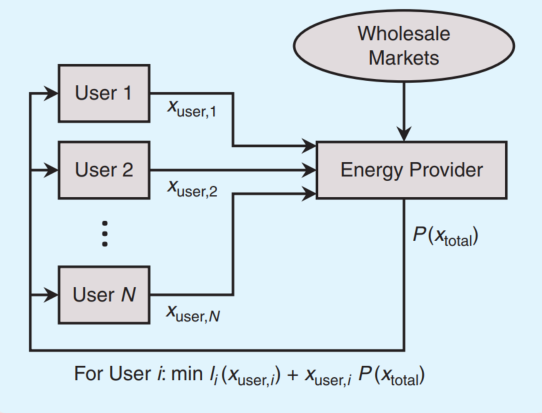
\includegraphics[height=1.5in]{figure/game/2-aggregative.png}
          \vspace{-6pt}
          \caption{ Aggregative Game}
      \end{figure}
      \column{6cm}
      \begin{equation}
        \begin{aligned}
        J_i = I_i(X_{user, i}) + X_{user, i} P(X_{total})
        \end{aligned}
        \end{equation}
    The objective of each electricity user is to minimize $J_i$which depends on its own energy consumption $X_{user,i}$ and the sum of all users’ energy consumption $X_{total}$.
  
    \item The aggregative game problems don't need to estimate all agents’ strategies, but require each agent to estimate the \textcolor[rgb]{0.00,0.00,1.00}{aggregation function} P.

    \end{columns}
\end{itemize}
\end{frame}


\begin{frame}
  \frametitle{\normalsize{Other Game Models}}\small
\begin{itemize}
  \item \textcolor[rgb]{1.00,0.00,0.00}{Other game models}
  
  There are also other distribute game models widely studied.
\end{itemize}

\begin{tabular}{cp{8cm}}% 其中,tabular是表格内容的环境;c表示centering,即文本格式居中;c的个数代表列的个数
	% \renewcommand\arraystretch{2}
  \toprule %[2pt]设置线宽     
  \centering
  Game models & Description \\
  \midrule %[2pt]  
 Zero-sum Games & The income of one player will inevitably lead to the loss of the other player. \\  \hline
  Potential Games & The change of single agent's local function and global function are equal.  $P\left(x_{i}, x_{-i}\right)-P\left(x_{i}^{\prime}, x_{-i}\right)=J_{i}\left(x_{i}, x_{-i}\right)-J_{i}\left(x_{i}^{\prime}, x_{-i}\right), \quad \forall x_{i}, x_{i}^{\prime} \in X_{i}$  \\
  \hline  Online Games & It refers to the adaptive decision making in repeated
  games. \\ \hline
  N-Coalition Games & Each coalition consisting of multiple agents collectively acts  as a virtual player to minimize the coalition cost function. \\
  \hline Gradient-Free Games &  The relation between the action variables and the cost functions is unknown. \\
  \bottomrule %[2pt]     
  \end{tabular}

  \breference
  \scriptsize
  [2]P. Yi, "A Survey on Noncooperative Games and Distributed Nash Equilibrium Seeking over Multi-Agent Networks
  " CAAI Artificial Intelligence Research 2022 Vol. 1 Issue 1 Pages 8-27
  \ereference
\end{frame}






\subsection[Nash equilibrium seeking algorithms]{Nash equilibrium seeking algorithms}\label{subsec:2-3}
\begin{frame}
  \frametitle{\normalsize\textsc{Consensus problem}}\transwipe
  
  \begin{itemize}
    \item In centrallized system, every agent know others' actions, so it's easy to calculates NE.
    \item In distributed systems, agents can only have an access to \textcolor[rgb]{0.00,0.00,1.00}{partial decision information}
    from its neighborhood agents, so they need communicate and exchange information through connected network to reach consensus.
    \item The \textcolor[rgb]{0.00,0.00,1.00}{leader-following} consensus technique has been widely used to reach consensus in distributed NE seeking
    \item The core idea of the strategy is that each player makes a local estimate of the unknown players’ actions by utilizing a leaderfollowing consensus protocol. 
    \begin{equation}
    \dot{y}_{i j}=-k_{i j}\left(\sum_{k=1}^{N} a_{i k}\left(y_{i j}-y_{k j}\right)+a_{i j}\left(y_{i j}-x_{j}\right)\right)
     \end{equation}

    where $y_{ij}$ represents agent i's estimation on agent j's action.
    \end{itemize}
  \end{frame}
  
\begin{frame}
  \frametitle{\normalsize\textsc{Nash equilibrium Seeking}}\transwipe
  
  \begin{itemize}
    \item Once consensus reached, it's easy to find NE just like centrallized systems.
    \item The gradient-like algorithm is adopted to update the players’ actions to reach NE.
     \begin{equation}
      \dot{x}_i  =-k_i \nabla_{x_i} J_i\left(y_i\right)
    \end{equation}
     It can replacing x in the gradients with $y_i$ for each agent, because agents update their actions based on their estimations.
    
     \item In fact,  agents' updation based on a combination of consensus and NE seeking module. To ensure the stability of the closed-loop system, a small positive parameter is included in the gradient part to ensure that the consensus part is faster than the gradient optimization part, thus forming a \textcolor[rgb]{0.00,0.00,1.00}{two time-scale structure}.
     
     \item The speed of consensus part is closely related to the communication network.
  \end{itemize}

  \end{frame}


\begin{frame}
    \frametitle{\normalsize\textsc{Graph Structure}}\transwipe
    
    \begin{itemize}
      \item When the communication graph is connected, the quasisteady state of the leader-following consensus part is $y_i = x$. But the \textcolor[rgb]{0.00,0.00,1.00}{convergence speed} is highly depends on graph's connectivity. The eigenvalue of graph's Laplacian matrix can used to convergence analysis.
      \item \textcolor[rgb]{1.00,0.00,0.00}{ Undirected Graph}\\
       Let $\lambda_{n}$ represent the eigenvalues of Laplacian matrix $\mathcal{L}$. When graph is connected, we have \\
      \begin{columns}[c]
        \column{6cm}
          \begin{figure}
              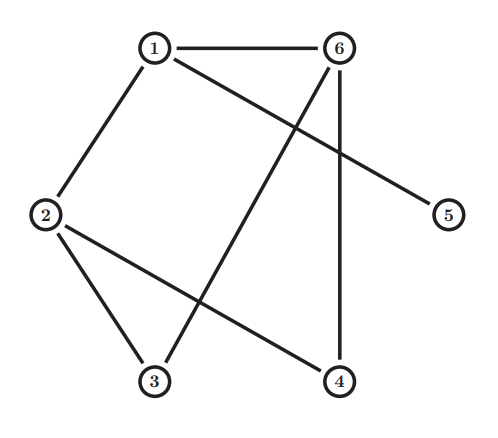
\includegraphics[height=1.2in]{figure/game/2-undirecti.png}
              \vspace{-6pt}
              \caption{ Undirected graph}
          \end{figure}
          \column{6cm}
          \begin{equation}
            \begin{aligned}
              \mathcal{L} &:=D-\mathcal{A} \\ 
              \lambda_{2} & > 0 \\
              \lambda_{1} & = 0 \\
              \lambda_{n} & \geq d_{\max }+1 \\ 
              0 \leq \lambda_{1} \leq \lambda_{2} &\leq \ldots \leq \lambda_{n}.\\ 
            \end{aligned}
            \end{equation}
         Where D is degree matrix, A is adjacency matrix. $\mathcal{L}$ is symmetric semi-positive definite, $d_{max}$ represents the maximum degrees in graph. 
        \end{columns}

    \end{itemize}
  
\end{frame}

\begin{frame}
  \frametitle{\normalsize\textsc{Graph Structure}}\transwipe
      \begin{itemize}
      \item \textcolor[rgb]{1.00,0.00,0.00}{ Directed Graph}\\
      \begin{columns}[c]
        \column{6cm}
          \begin{figure}
              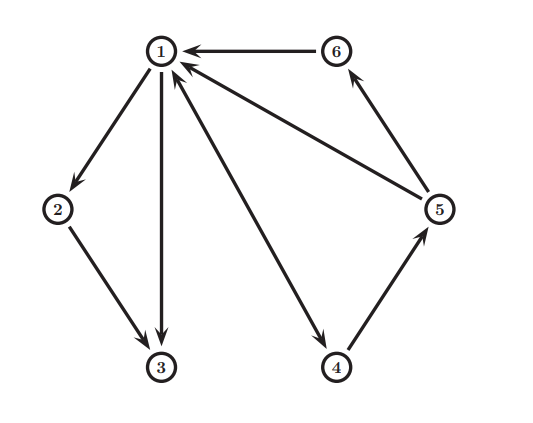
\includegraphics[height=1.2in]{figure/game/2-directi.png}
              \vspace{-6pt}
              \caption{ Directed graph}
          \end{figure}
          \column{6cm}
          \begin{equation}
            \begin{aligned}
              &\mathcal{L} :=D_{in} -\mathcal{A} \\ 
              &R \mathcal{L}  +\mathcal{L}^{T} R \geq 0 \\
              &R =\operatorname{diag}\left(r_{1}, \cdots, r_{N}\right), r_i \ge 0\\
              &r^{T} \mathcal{L}=0 \text { and } r^{T} \mathbf{1}=1 \\ 
            \end{aligned}
            \end{equation}
        
        \item Where $D_{in}$ is in-degree matrix. r is left eigenvector of $\mathcal{L}$ associated with the zero eigenvalue.
        \item When graph is strong connected, r is unique. 
        \item The second equation widely used to convergence analysis, because $\mathcal{L}$ is indefinite matrix.
        \end{columns}
    \end{itemize}

\end{frame}



\begin{frame}
  \frametitle{\normalsize{Generalized Nash Equilibrium Seeking}}\small
  
\begin{itemize}

  \item For GNE seeking (in addition to estimating the actions), the multipliers of all players for the same constraint must be synchronized since finding a GNE where the Lagrangian multiplier of each player is different may be extremely hard.
  \begin{equation}
  \begin{aligned}
    \dot{x}_{i} & =-k_{i}\left(\nabla_{x_{i}} J_{i}\left(y_{i}\right)+\lambda_{i} \nabla_{x_{i}} g\left(y_{i}\right)\right) \\
    \dot{\lambda}_{1} & =k_{1} \lambda_{1} g\left(y_{1}\right)\\
    \dot{\lambda}_{i} & =-\gamma_{i} \sum_{k=1}^{N} a_{i k}\left(\lambda_{i}-\lambda_{k}\right), \\
    \dot{y}_{i j} & =-w_{i j} \sum_{k=1}^{N} a_{i k}\left(y_{i j}-y_{k j}\right), \quad j \in \mathcal{V} \backslash\{i\}
  \end{aligned}
  \end{equation}
  \item  player 1  calculates the common multiplier using second equation, and all of the
  other players estimate this multiplier using a leader-following consensus algorithm in third equation. In addition, last equation is
  for action estimation.
\end{itemize}
\end{frame}


\begin{frame}
  \frametitle{\normalsize{Nash Equilibrium Seeking in  Aggregative Games}}\small


\begin{itemize}
  \item To achieve distribute NE seeking, different from general Nash games, the aggregative game problem does not need to estimate all agents’ strategies, but only requires
  each agent to estimate the sum of players' local function.

  \begin{equation}
  \begin{aligned}
    \dot{x}_{i}&=\mathcal{P}_{\Omega_{i}}\left(x_{i}-G_{i}\left(x_{i}, \eta_{i}\right)-\frac{\gamma}{N} A_{i}^{\top} \lambda_{i}\right)-x_{i,} \\
    \dot{\lambda}_{i}&=\beta \sum_{j \in \mathcal{N}_{i}} \operatorname{sgn}\left(\lambda_{j}-\lambda_{i}\right)+\gamma\left(A_{i} x_{i}-b_{i}\right), \\
    \dot{\zeta}_{i}&=\alpha \sum_{j \in \mathcal{N}_{i}} \operatorname{sgn}\left(\eta_{j}-\eta_{i}\right), \\
    \eta_{i}&=\zeta_{i}+\phi_{i}\left(x_{i}\right),  
  \end{aligned}
  \end{equation}

  \item 
   $G_{i}\left(x_{i}, \eta_{i}\right):=\left.\nabla_{x_{i}} J_{i}(x)\right|_{\sigma(x)=\eta_{i}}, A=\left[A_{1}, \ldots, A_{N}\right], b=\sum_{i=1}^{N} b_{i} $.\\
  x represents the players' actions, $\lambda$ is the multiplier, $\zeta$ used to estimate others local cost function and $\eta$ is the sum of cost function.
\end{itemize}
\breference
\scriptsize
[3] G. Hu, ``Distributed Nash Equilibrium Seeking: Continuous-Time Control-Theoretic Approaches''  \emph{IEEE Control Systems Magazine }, 2022 Vol. 42 Issue 4 Pages 68-86.
\ereference
\end{frame}

\begin{frame}
\frametitle{\normalsize\textsc{Related Work}}\transwipe 
    
\begin{itemize}
    \item Here are related work about distributed Nash equilibrium seeking in different game structures and  we mainly focus on continuous-time.\\

      \begin{tabular}{ccccc}     \footnotesize
        \diagbox{Models}{Structure} & Constraint&  Undirected & Directed  & Varing \\
        \hline
        Generalized games & Type I/II/III/IV  & \checkmark & \checkmark &    \\
        \hline
        \multirow{2}{4em}{Aggregative games }&  Type I  &\checkmark & \checkmark& \\
        & Type II  &\checkmark &  &  \\ 

        \hline
        Zero-Sum games & NA &\checkmark & \checkmark &     \\
        \hline
        N-Coalition  games & NA  & \checkmark & \checkmark & \checkmark  \\

        \bottomrule %[2pt]     
      
    \end{tabular}

    \end{itemize}
    \breference
    \scriptsize
    [4]Z. Li and Z. Duan, Cooperative Control of Multi-Agent Systems:
    A Consensus Region Approach. Boca Raton, FL, USA: CRC Press, 2017  \par
    [5]M. Ye, Q.-L. Han, L. Ding and S. Xu, Distributed Nash Equilibrium Seeking in Games With Partial Decision Information: A Survey, IEEE 2023 Pages 1-18
    \ereference
  \end{frame}
